\clearpage
\section{Oblivious Transfer with Discrete Variables}

\begin{tcolorbox}	
\begin{tabular}{p{2.75cm} p{0.2cm} p{10.5cm}} 	
\textbf{Student Name}  &:& Mariana Ramos\\
\textbf{Starting Date} &:& September 18, 2017\\
\textbf{Goal}          &:& Oblivious transfer implementation with discrete variables.
\end{tabular}
\end{tcolorbox}

Oblivious Transfer (OT) is a fundamental primitive in multi-party computation. The one-out-of-two OT consists in a communication protocol between Alice and Bob. At the beginning of the protocol Alice has two messages $m_1$ and $m_2$ and Bob wants to know one of them, $m_b$, without Alice knowing which one, i.e. without Alice knowing $b$, and Alice wants to keep the other message private, i.e. without Bob knowing $m_{\bar{b}}$. therefore two conditions must be fulfilled:
\begin{enumerate}
	\item{The protocol must be concealing, i.e at the beginning of the protocol Bob does not know nothing about the messages sent by Alice, while at the end of the protocol Bob will learn the message $b$ chose by him.}
	\item{The protocol is oblivious, i.e Alice cannot learn anything about bit $b$ and Bob cannot learning nothing about the other message $m_{\bar{b}}$.}
\end {enumerate}

\subsection{OT Protocol Detailed}

 First of all, it is important to set the initial conditions of Bob and Alice's knowledge.

In general, the first step is to establish for both Alice and Bob the message length $s$ and the parameter $k$, which is multiplicative factor of message's length.
In this case, lets assume message's length $s=4$ and a multiplicative factor $k=2$.

 In addition, both Alice and Bob know the following correspondence, where $+$ corresponds to \textit{Rectilinear Basis} and $\times$ corresponds to \textit{Diagonal Basis}:

\begin{table}[H]
\centering
\begin{tabular}{c|c}
\textbf{\textit{Basis}}         &  \\ \hline
 0 & $+$ \\
 1 & $\times$ \\
\end{tabular}
\end{table}

Secondly both Alice and Bob also know the bit correspondence for each direction for each basis. For \textit{Rectilinear basis}, "$+$":

\begin{table}[H]
\centering
\begin{tabular}{c|c}
            & Basis "+" \\ \hline
 0 & $\to$ \\
 1 & $\uparrow$ \\
\end{tabular}
\end{table}

and for \textit{Diagonal Basis}, "$\times$":

\begin{table}[H]
\centering
\begin{tabular}{c|c}
      & Basis "$\times$" \\ \hline
 0 & $\searrow$ \\
 1 & $\nearrow$ \\
\end{tabular}
\end{table}

Third, only Alice knows information about messages $m_{1}$ and $m_{2}$.
In this case, lets assume she sets the two messages $m_{1} = \{0 0 1 1\}$ and $m_{2} = \{0 0 0 1\}$.

\begin{enumerate}
  \item Alice randomly generate a bit sequence with length $k.s$ being, in this case, $k=2$ and $s=4$ and both were defined at the beginning of the protocol.
      Therefore, she must define two sets $S_{A1}$, which contains the basis values, and $S_{A2}$, which contains the key values.

      In that case, lets assume she gets the following sets $S_{A1}$ and $S_{A2}$:
      $$S_{A1} = \{0,1,1,0,0,1,0,1 \}$$
      $$S_{A2} = \{1,1,0,0,0,1,0,0 \}$$

  \item Next, Alice sends to Bob throughout a quantum channel $ks$ photons encrypted using the basis defined in $S_{A1}$ and according to the keys defined in $S_{A2}$.

      In the current example, Alice sends the photons, throughout a quantum channel, according to the following basis and keys:

      $$S_{AB} = \{\uparrow, \nearrow, \searrow, \to, \to, \nearrow, \to, \searrow \}$$

  \item Bob also randomly generates $ks$ bits according to the basis through which he will measure the photons sent by Alice and he fills an array $S_{B1}$ with the basis chosen by him. In this example, lets assume:

  $$S_{B1} = \{0,1,0,1,0,1,1,1 \}$$

  \item When Bob receives photons from Alice, he measures them using the basis defined in $S_{B1}$.
  In the current example, we assumed that $S_{B1}$ is the following set:
  $$\{ +,\times,+,\times,+,\times, \times, \times \}$$
  In this follow-up he will get $ks$ results. Some of them Bob is $100\%$ sure he was succeeded and others he may be succeeded or not with a probability of $\frac{1}{2}$. The values which he is not sure about are underlined in the following sequence:
  $$S_{B1\prime} = \{1,1,\underline{0},\underline{1},0,1,\underline{1},0 \}$$

  \item Once Alice has received the confirmation of measurement from Bob, she sends throughout a classical channel the basis which she has used to codify the photons, which in this case we assumed $S_{A1} = \{0,1,1,0,0,1,0,1\}$.

  \item In order to know which photons were measured correctly, Bob does the operation $S_{B2}=S_{B1} \oplus S_{A1}$.
      In the current example the operation will be:

  \begin{table}[H]
    \centering
    \begin{tabular}{c|c c c c c c c c}
     $S_{B1}$ & 0 & 1 & 0 & 1 & 0 & 1 & 1 & 1 \\
     $S_{A1}$ & 0 & 1 & 1 & 0 & 0 & 1 & 0 & 1 \\ \hline
     $\oplus$ & 1 & 1 & 0 & 0 & 1 & 1 & 0 & 1
    \end{tabular}
    \end{table}

      In this way, Bob gets $$S_{B2} = \{1,1,0,0,1,1,0,1 \}$$. The values "$1$" correspond to the values he measured correctly and "$0$" to the values he wrongly measured.

       Next, Bob sends to Alice through a classical channel information about the minimum number between "ones" and "zeros", i.e $$n=min(\#0,\#1)=3$$ where $\#0$ represents the minimum number of zeros and $\#1$ the minimum number of ones. Function $min(a,b)$ counts the number of \textit{a}, $n_{a}$, and the number of \textit{b}, $n_{b}$ and if $n_{a}<n_{b}$ the function will takes $n_{a}$ as result and $n=n_{a}$, otherwise $n=n_{b}$.

  \item If $n<s$, being \textit{s} the message's size, Alice and Bob will repeat the steps from $1$ to $7$.

  \item Lets assume for the values set which contains the results of Bobs measurements $S_{B1\prime}$ we have the following sequence being underlined values those which Bob is not $100\%$ sure about, having a probability of success about $\frac{1}{2}$ :

   $$S_{B1\prime}= \{1,1,\underline{0},\underline{0},0,1,\underline{0},0,\underline{1},0,\underline{0},\underline{0},0,0,\underline{1},1 \}$$

    At Alice's side the new sets $S_{A1}$, which contains the basis values, and $S_{A2}$, which contains the key values, will be the following:

    $$S_{A1}=\{0,1,1,0,0,1,0,1,1,1,0,0,1,1,1,0 \}$$ $$S_{A2}=\{1,1,0,0,0,1,0,0,1,0,1,0,0,0,1,1 \}$$

    Finally, for $S_{B2}=S_{B1} \oplus S_{A1}$ Bob gets the following sequence:

    $$S_{B2}= \{1,1,0,0,1,1,0,1,0,1,0,0,1,1,0,1 \}$$

  \item At this time, Bob sends again to Alice through a classical channel the minimum number between "ones" and "zeros" $n=min(\#0,\#1)$. In this case, $n$ is equal to $7$ which is the number of zeros.

  \item Alice checks if $n>s$ and reveals to Bob that she already knows that $n>s$. In this case, $n=7$ and $s=4$ being $n>s$ a valid condition.

  \item Next, Bob defines two new sets, $I_{1}$ and $I_{0}$ where one contains $s$ positions of measurements that Bob has succeeded and other contains $s$ positions of measurements that Bob was wrong about, respectively.

  In this example, Bob defines two sequences with size $s=4$:
  $$I_{0}=\{3,4,7,11 \}$$
  and $$I_{1}= \{2,5,6,13 \}$$ where $I_{0}$ is the sequence of positions in which Bob was wrong and $I_{1}$ is the sequence of positions in which Bob was right.

  Thus, if Bob wants to know $m_{1}$ he must send to Alice throughout a classical channel the set $\{I_{1},I_{0} \}$, otherwise if he wants to know $m_{2}$ he must send to Alice throughout a classical channel the set $\{I_{0},I_{1} \}$.

  \item Lets assume Bob sent $\{I_{1},I_{0} \}$.
   Alice defines two encryption keys $K_{1}$ and $K_{2}$ using the values in positions defined by Bob in the set sent by him. In this example, lets assume: $$K_{1}=\{1,0,1,0\}$$ $$K_{2}=\{0,0,0,1\}$$

   Alice does the following operations:
   $$m = \{m_{1}\oplus K_{1}, m_{2} \oplus K_{2} \}$$

   \begin{table}[H]
    \centering
    \begin{tabular}{c|c c c c c c c c}
     $m_{1}$ & 0 & 0 & 1 & 1 \\
     $K_{1}$ & 1 & 0 & 1 & 0 \\ \hline
     $\oplus$ & 1 & 0 & 0 & 1
    \end{tabular}
    \end{table}

   \begin{table}[H]
    \centering
    \begin{tabular}{c|c c c c c c c c}
     $m_{2}$ & 0 & 0 & 0 & 1 \\
     $K_{2}$ & 0 & 0 & 0 & 1 \\ \hline
     $\oplus$ & 0 & 0 & 0 & 0
    \end{tabular}
    \end{table}

    Adding the two results, $m$ will be: $$m=\{1,0,0,1,0,0,0,0\}$$.

   After that, Alice sends to Bob the encrypted message $m$ through a classical channel.

  \item When Bob receives the message $m$, in the same way as Alice, Bob uses $S_{B1\prime}$ values of positions given by $I_{1}$ and $I_{0}$ and does the decrypted operation. In this case, he does following operation:

      \begin{table}[H]
        \centering
        \begin{tabular}{c|c c c c c c c c}
         $m$ & 1 & 0 & 0 & 1 & 0 & 0 & 0 & 0 \\
             & 1 & 0 & 1 & 0 & 0 & 1 & 1 & 0 \\ \hline
         $\oplus$ & 0 & 0 & 1 & 1 & 0 & 1 & 1 & 0 \\
        \end{tabular}
        \end{table}

      The first four bits corresponds to message 1 and he received $\{0,0,1,1\}$, which is the right message $m_{1}$ and $\{0,1,1,0\}$ which is a wrong message for $m_{2}$.


\end{enumerate}

\subsection{OT Protocol - Potential Problems}
There are two potential problems with the protocol described above:
\begin{enumerate}
  \item In step $5$ Bob may says to Alice that he has already measured the photon and it could be a lie.

  \item In step $10$ Bob may uses some values of $I_{1}$ in $I_{0}$ of positions which he knows are right in order to know correct information about message $m_{2}$.
\end{enumerate}

This problems can hopefully be solved using \textit{Bit Commitment} through \textit{Hash Functions}.

\subsection{Simulation}

First of all, the protocol will be simulated and then a experimental setup will be built in the laboratory.

\begin{figure}[H]
	\centering
	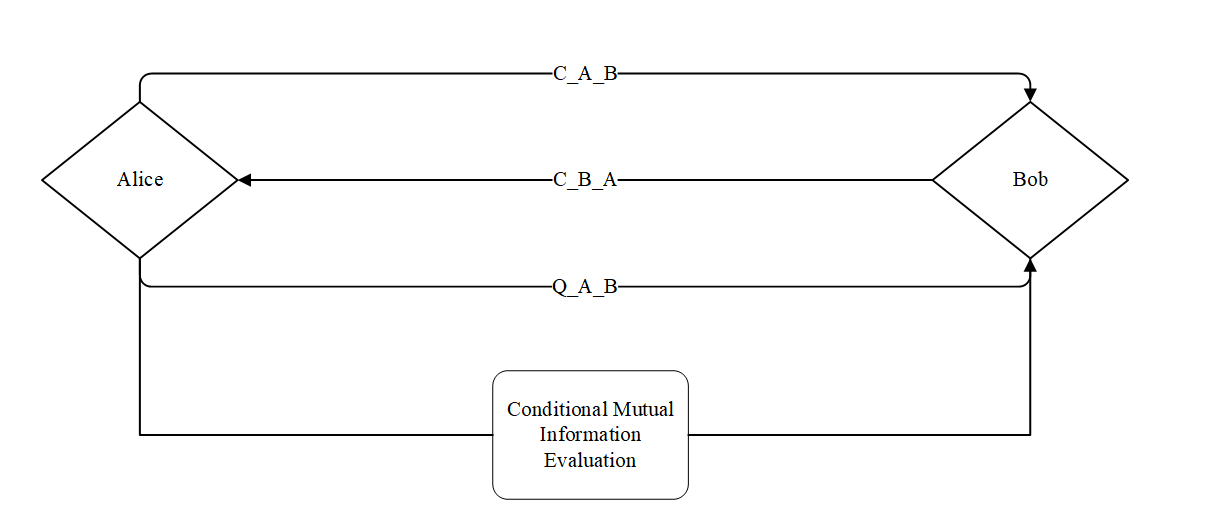
\includegraphics[width=1.0\textwidth, height=8cm]{./sdf/ot_with_discrete_variables/figures/Simulation_diagram_1.png}
	\caption{Simulation diagram at a top level}\label{toplevelsimulation}
\end{figure}

As one may see in figure \ref{toplevelsimulation} this simulation will have three top level blocks. Two of them are Alice and Bob and they are connected through two classical channels and one quantum channel. In addition, a third block will be performed for the calculation of \textit{Mutual Information}. The mutual information (MI) between Alice and Bob is defined in terms of their join distribution.

\begin{figure}[H]
	\centering
	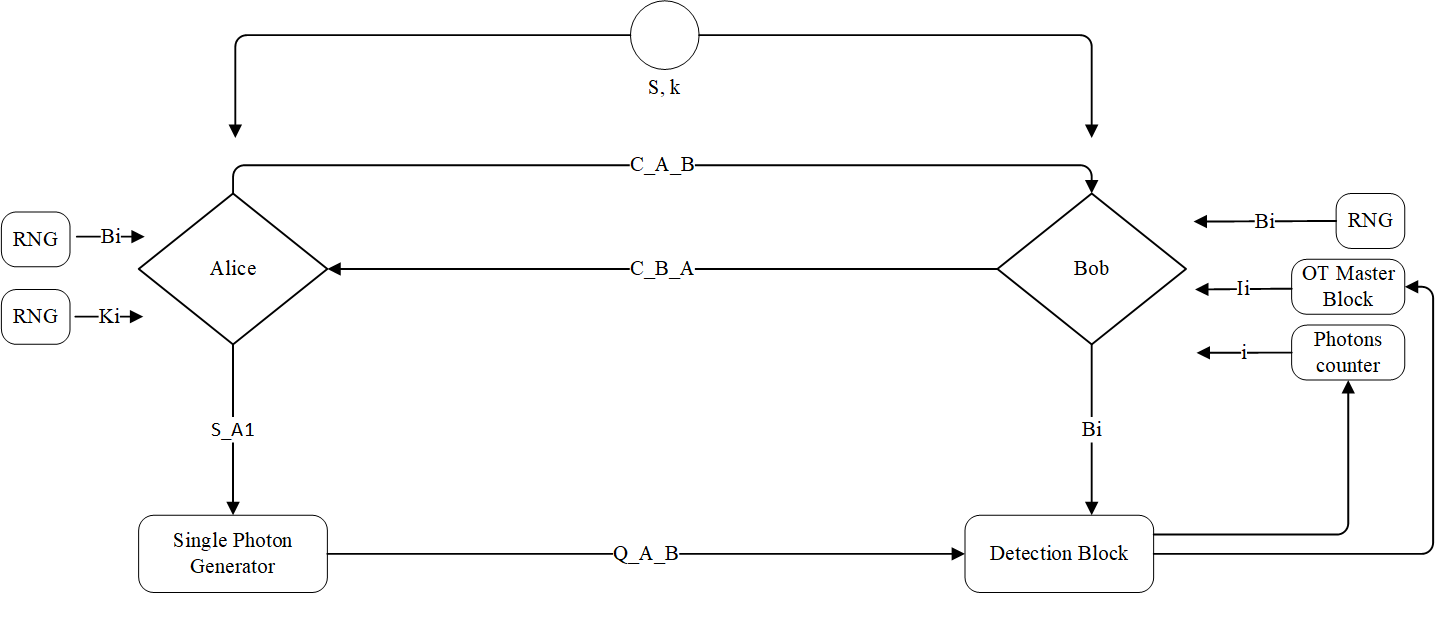
\includegraphics[width=1.0\textwidth, height=8cm]{./sdf/ot_with_discrete_variables/figures/Simulation_diagram.png}
	\caption{Simulation diagram - blocks}\label{blocksimulation}
\end{figure}

In figure \ref{blocksimulation} is presented the block diagram of the simulation that will be performed. There are two sides (Alice and Bob) and three channels throughout which they will communicate. 
At the beginning of the protocol Alice and Bob must know two values: message's size, s, and a multiplicative factor, k.
Furthermore, Alice must have two blocks, \textit{RNG - Random Number Generate}, for randomly picks the basis $B_{i}$ and the keys $K_{i}$. In a similar way, Bob also has one \textit{RNG - Random Number Generate} for randomly chooses in which basis he will measure the photons sent by Alice. In addition, Bob has one \textit{OT Master Block} to analyse the data and picks two more sub-sets $I_{0}$ and $I_{1}$ and a \textit{Photons counter} which has i as output in order to send to Alice the number of photons which Bob has received through the Quantum channel. 
Moreover, Alice must have a block for \textit{Single Photon Generator} which receives information through "$S_A1$" channel about the basis and keys to encrypt the photons and then send them to Bob using the Quantum channel.

In general, the simulation must have two Classical channels, one from Alice to Bob and other from Bob to Alice through which they change all the information about basis. Third channel is used only in one direction, from Alice to Bob, and Alice sends the photons to Bob through this channel.

\subsection{Experimental}
In figures \ref{quantumchannelcommunication1} and \ref{quantumchannelcommunication2} are presented the experimental setup to be performed in the lab. Starting with Alice's side and then Bob's side.

\begin{figure}[H]
	\centering 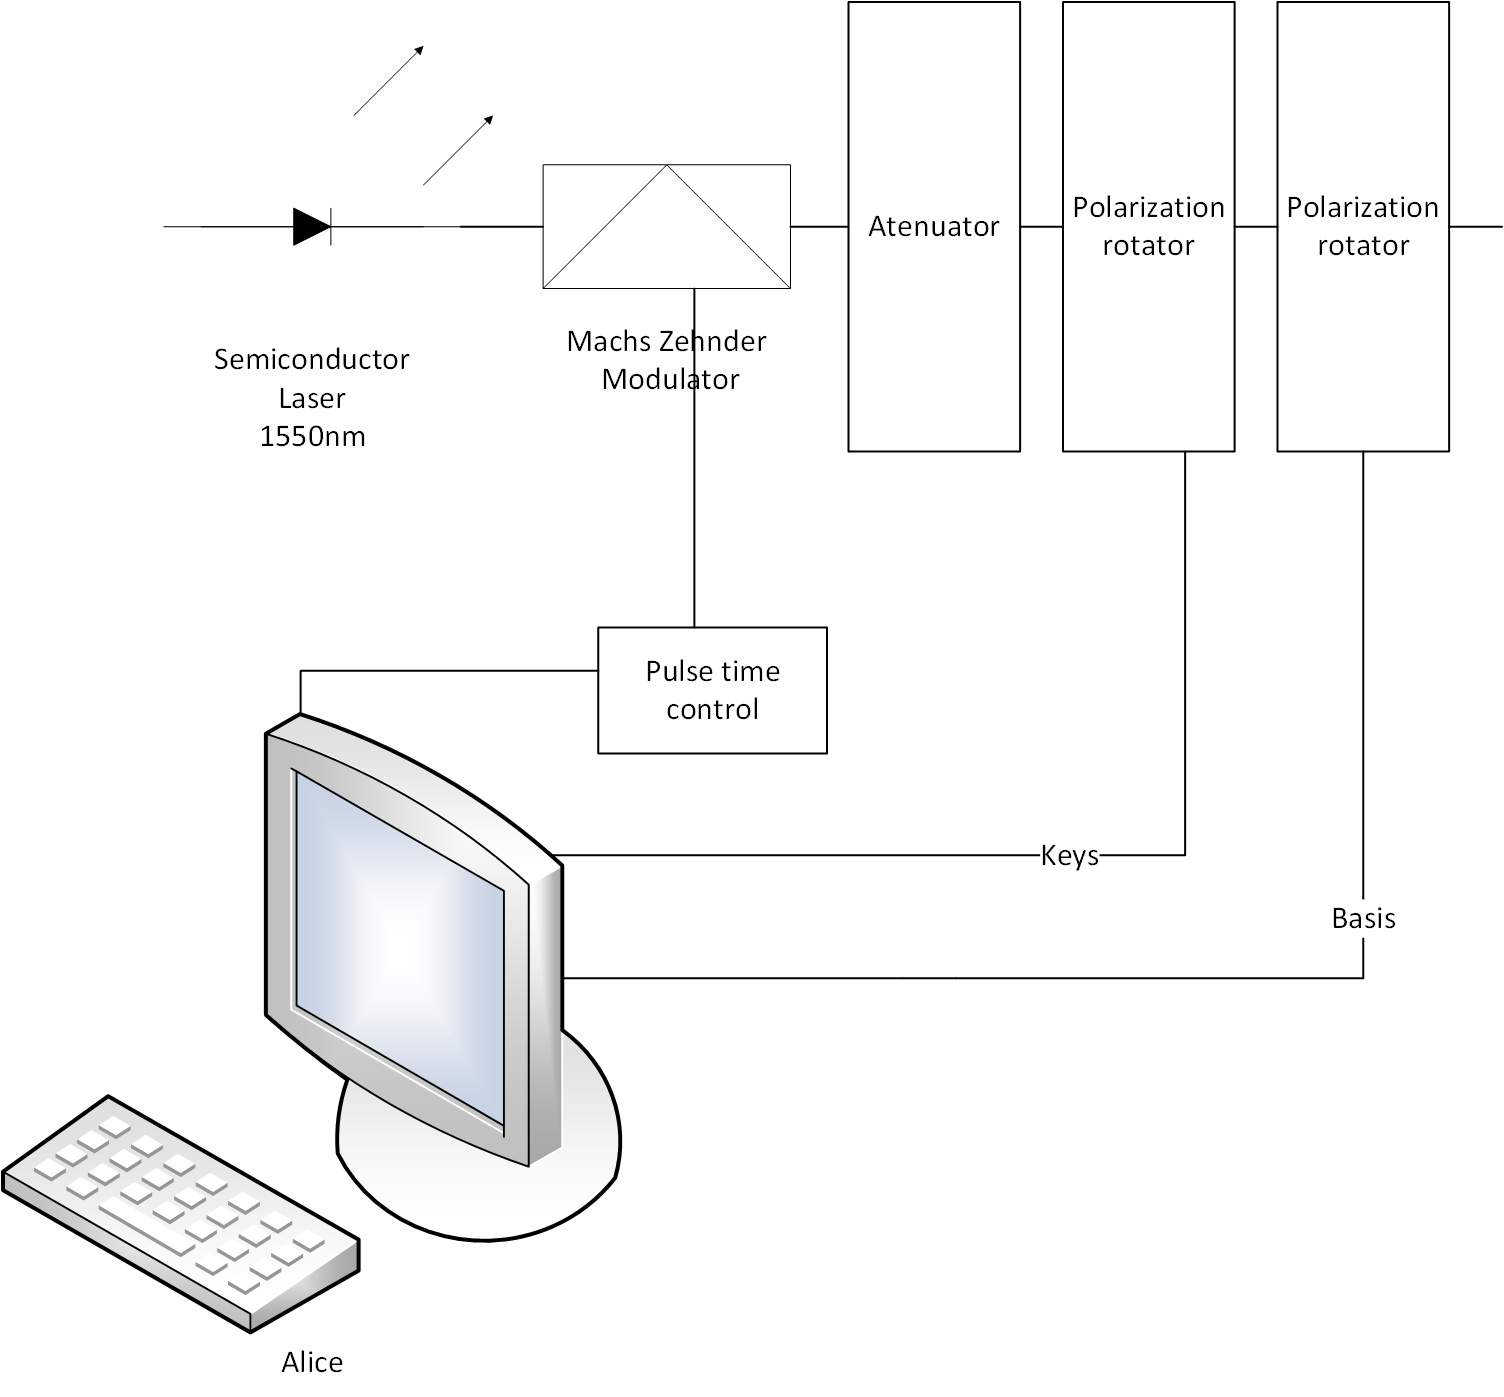
\includegraphics[width=0.8\textwidth,height=8cm]{./sdf/ot_with_discrete_variables/figures/OT_experimental_alice.png}
	\caption{Quantum communication diagram - Alice's side}\label{quantumchannelcommunication1}
\end{figure}

\begin{figure}[H]
	\centering 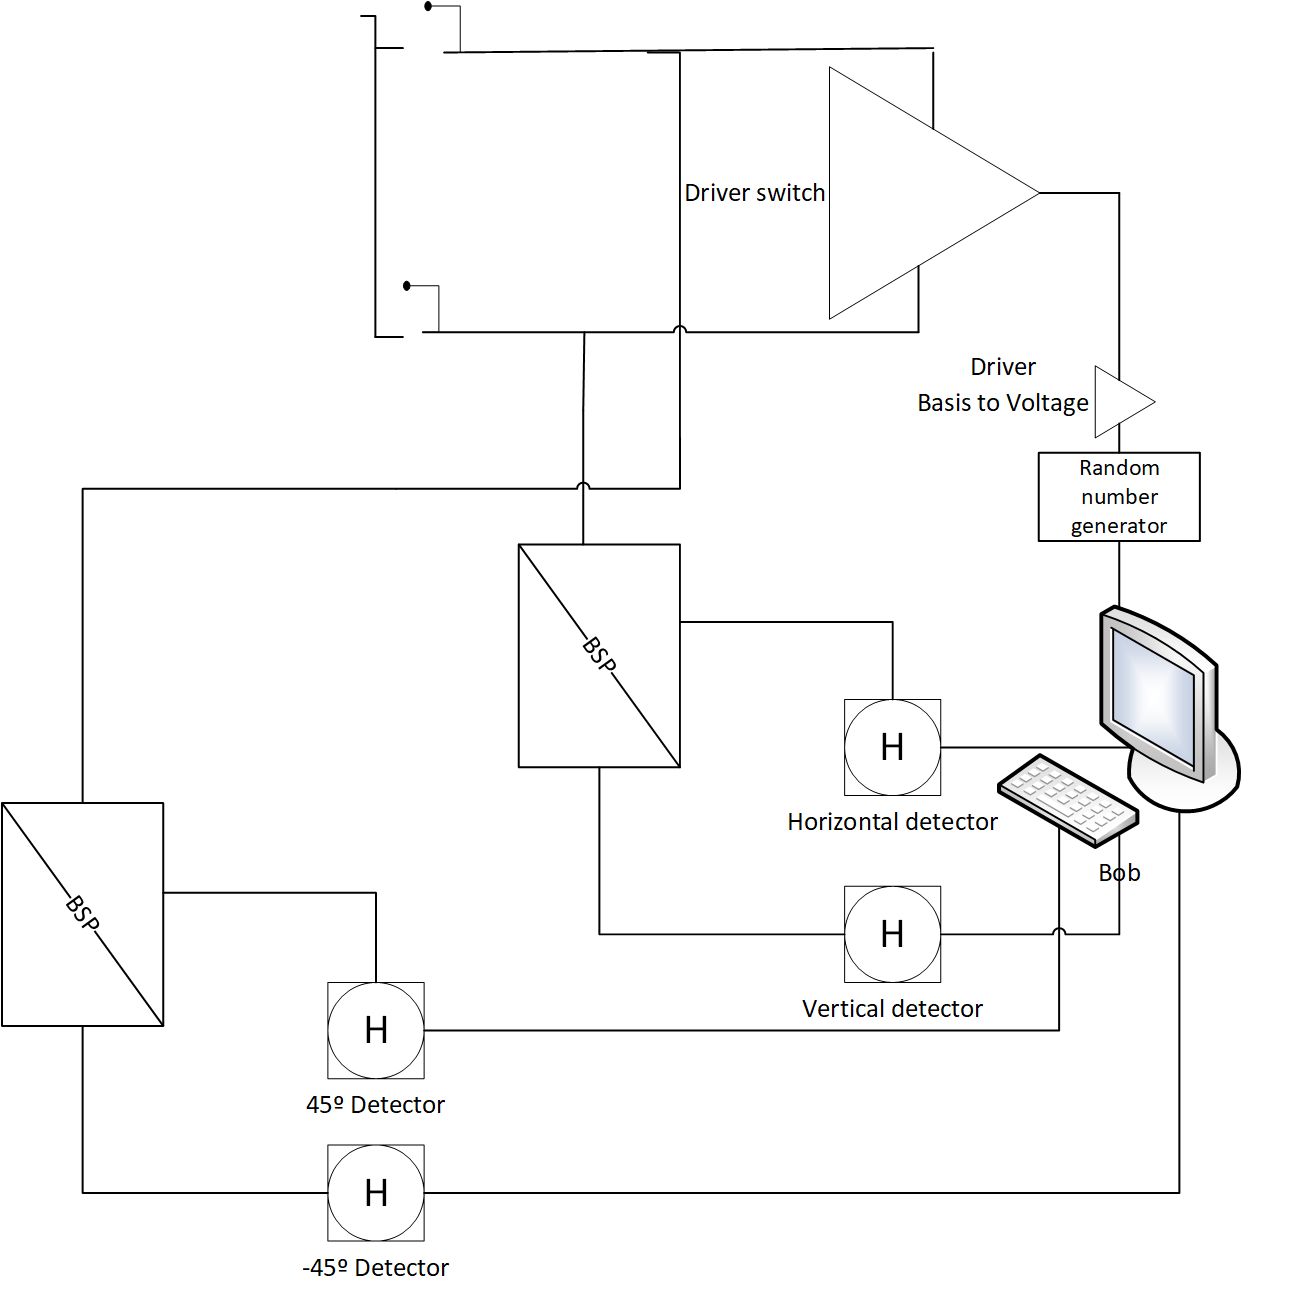
\includegraphics[width=0.8\textwidth,height=9cm]{./sdf/ot_with_discrete_variables/figures/OT_experimental_bob.png}
	\caption{Quantum communication diagram - Bob's side}\label{quantumchannelcommunication2}
\end{figure} 
